% TODO_ The following notions must have been introduced before:
% - What a DH key exchange is
% - CanFlow should be introduced in the background
% - Forward secrecy and post-compromise security (via state) must have been introduced before
% - Versions must have been introduced in the DY* chapter of the Background
% - The fractional permission system must have been introduced in the Background chapter
% - The Mem predicate must have been introduced in the Background chapter

\chapter{Design}

% We want to extend the work of Arquint et al.\ \cite{} to support the safe deletion of old data.
% Practically, we want to extend their Reusable Verification Library in order to provide someone verifying a protocol implementation with the possibility of proving security properties like post-compromise security.

% Explain that we will use "the developer" to mention the person who will use the library to verify a protocol implementation

\section{Overview}
\label{sec:overview}

This section gives an overview to better understand our goal and the high-level idea of our methodology to achieve it.
With the aim of verifying properties like forward secrecy and post-compromise security for a protocol implementation, we need to model the fact that some ephemeral values should only exist for a limited amount of time.

We start by explaining the goal of our methodology by introducing a relevant protocol, the Diffie-Hellman Ratchet, and the security properties we want to prove for it.
Then, we explain how we introduce a notion of temporality in the methodology, by adding  \emph{versions}, which define fine-grained time frames during which some values are accessible.
Finally, because versions specify that a value should only be able to exist in some time frame, we reason about how to enforce that it is deleted before this time frame ends.

\subsection{Goal}
\label{sec:goal}

We aim to verify protocol implementations that frequently renew their communication keys to provide strong security properties.
A notable example is the Signal Double Ratchet protocol. To make our point simpler, we consider a simplified version of this protocol, the Diffie-Hellman Ratchet.

\subsubsection{Diffie-Hellman Ratchet}
\label{sec:diffie-hellman-ratchet}

The Diffie-Hellman (DH) Ratchet is a continuous key agreement protocol, which repeatedly performs Diffie-Hellman key exchanges to encrypt each message with its own key.
It is presented in Figure \ref{fig:dh-ratchet}.

\begin{figure}
    \centering
    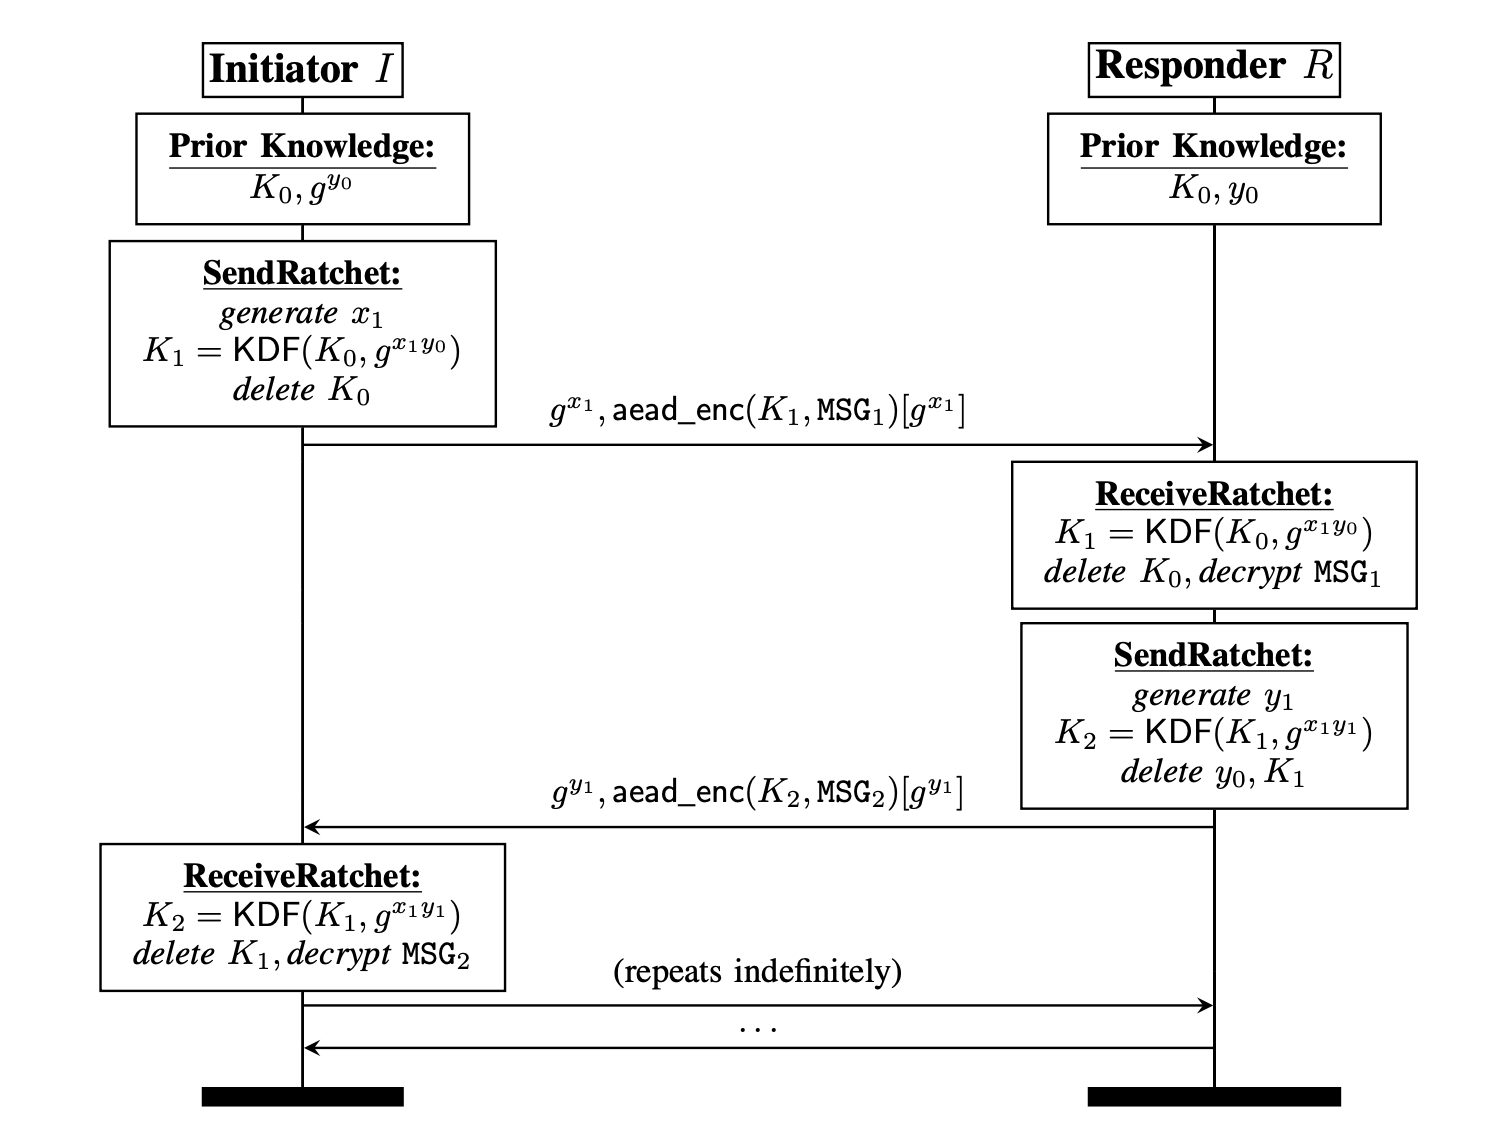
\includegraphics[width=1.0\textwidth]{figures/DH-ratchet.png}
    \caption{Diffie-Hellman Ratchet protocol.}
    \label{fig:dh-ratchet}
\end{figure}
\todo{Change the figure to use my own protocol figure, and modify the caption to explain the figure more in detail}

The protocol starts with an established communication key $K_0$, mutually shared by both participants.
The initiator uses the responder's public key and a newly generated secret key to compute a Diffie-Hellman secret. 
This newly generated secret is then blended with $K_0$, resulting in the derivation of a fresh communication key $K_1$.
This step of generating a new key from the previous one is called a \emph{ratcheting step}.
Then, $K_1$ is used to encrypt the message sent to the responder, accompanied by the initiator's new public key.
The responder can obtain the Diffie-Hellman shared secret and take the same ratcheting step to obtain $K_1$, then use it to decrypt the message.
This iterative process continues for each message, with the initiator and the responder continuously ratcheting.

After this ratcheting process has been performed and has given us a communication key $K_n$, the previous key $K_{n-1}$ is no longer needed and is deleted.

\subsubsection{Security properties}
\label{sec:security-properties}
% \todo{This may move to the Background chapter}

\paragraph{Forward secrecy.}
\label{sec:forward-secrecy}

The DH Ratchet protocol is designed to be secure against an attacker recording all previous encrypted messages and obtaining a shared secret or a communication key at some point.
If the attacker compromises a participant, for example, Alice, they may be able to decrypt some messages using the keys and secrets stored in Alice's memory. If Alice keeps storing all previous secrets and session keys, then the attacker would be able to decrypt all previous messages that they previously observed on the network. This is why it is crucial for Alice to delete previous secrets and communication keys as soon as she has derived the new ones.
Indeed, if previous keys are correctly deleted from Alice's memory, then the attacker may only be able to decrypt the last message and not all previous ones.

Therefore, the DH Ratchet protocol satisfies forward secrecy. This property is enabled by two main factors: cryptographically preventing past communication keys from being derived from the long-term secret and current communication keys, and securely deleting previous keys.

\paragraph{Post-compromise security.}
\label{sec:post-compromise-security}

Additionally, the DH Ratchet protocol is designed to be \emph{self-healing}, meaning that it should allow communication to resume securely at some point after a compromise. This is the property of post-compromise security.
Recall that post-compromise security is not achievable after the \emph{unrestricted} compromise of a participant, but we instead consider that some secret data remains available exclusively to the participants after the compromise (post-compromise \emph{via state}).
In the DH Ratchet protocol, we consider that the attacker compromised Alice's $K_n$ communication key \emph{after} she derived the new $K_{n+1}$ key. At this point, the attacker cannot obtain $K_{n+1}$ because they cannot have access to the new Diffie-Hellman shared secret. 

Therefore, all future communication keys are safe from the attacker, so the DH Ratchet protocol satisfies post-compromise security via state.
Although post-compromise security is not directly related to secure deletion, it requires fine-grained reasoning about the data occurring in a participant's state at a particular point in time.

Our methodology to prove these two strong security properties requires a notion of temporality because we have to specify the lapses of time during which certain keys are available. Outside these lapses, keys must not be present in memory because they have either not been generated yet or have already been securely deleted.

\subsection{Versions}
\label{sec:versions}

In order to introduce a notion of temporality, we introduce a \emph{version} identifier, similarly to what is done in DY*. Each participant's session is given a version field, initially set to $0$, which keeps track of the current version of the protocol.
Each term, e.g. a key or a nonce, is assigned a secrecy label stating who can access it. While these labels could previously only be defined from participant or session identifiers, we now allow them to be defined from version identifiers as well. Formally, a version identifier is a triplet identifier of the form $(p, s, v)$, where $p$ is a participant, $s$ is a session, and $v$ is a version.

We distinguish two cases: \emph{versioned} and \emph{unversioned} terms.
A term is said to be versioned if it is made to be accessible only in one or several specific versions, while it is said to be unversioned if it is made to be accessible by a participant or a session. 
An unversioned term accessible by some session is therefore accessible by all versions of that session.
Additionally, we define a $i$-versioned term as a versioned term that is accessible in version $i$.

The existing methodology already enforces that unversioned terms can only be accessed by participants or sessions allowed by their secrecy label.
A key property of our methodology extension is to ensure that versioned terms can only be accessed when the session is in a version allowed by their secrecy label. Intuitively, this means that an ephemeral key, defined as a versioned value, should only be accessible during a limited time frame defined by the versions allowed by its secrecy label.

On a high level, this requires two kinds of checks.
First, we enforce when creating a versioned term that it should be readable in the current version of the protocol.
Second, we enforce that when increasing the version of a session, all versioned terms that are no longer accessible in the new version are deleted.
While the first check can be easily implemented similarly to the existing check for unversioned terms, the second check requires more work. Indeed, using Gobra, there is no trivial way to check a condition on \emph{all versioned terms}.

This second check is crucial as it will drive the deletion mechanism, and ensure that ephemeral keys are deleted when they are no longer needed. Let us discuss this in more detail.

\subsection{Enforcing deletion of old data}
\label{sec:enforcing-deletion-of-old-data}

Before increasing the version of a session, we have to securely delete all versioned terms that are no longer accessible in the new version. By doing so, we more generally ensure that terms are only accessible in the time frames allowed by their secrecy label.

While this problem has already been solved in DY*, we show that their approach is not applicable in our case. We then introduce our approach on a high level.

\subsubsection{Existing approach in DY*}
\label{sec:existing-approach-in-dy}
\todo{This may move to the Background chapter}

In DY*, a participant uses a storage API to store all of its knowledge on the trace.
In particular, it stores the knowledge of ongoing sessions into an array, composed of each serialized session state.
Each session is given a version number.
To update some session state, the participant first reads and deserializes the corresponding session state from the array, then modifies it, and finally serializes and stores it back into the array.
The participant can also update and increment the version number at this point.

Upon serialization and storage of the updated state, an invariant is checking that only values still accessible in the session's version are stored.
Thus, only data from the current version can be stored, ensuring that neither outdated keys nor future keys are present in memory.
Building on this, they can prove forward secrecy and post-compromise security for protocols like Signal.

However, DY* does not enforce that outdated keys are \emph{securely} deleted from memory. They only show that they are not present in the current scope, but outdated keys are not explicitly zeroed out from memory.
Moreover, this solution does not apply to existing implementations because their state is not stored on a trace, making it impossible to express such an invariant.
Furthermore, DY* enforces the invariant over state only at certain time points, namely when the state is stored on the trace, without taking into account the state in-between.

\subsubsection{Our approach}
\label{sec:our-approach}

As we cannot simply iterate over the full session state to remove outdated keys like in DY*, we present a new approach to enforce that versioned values are deleted before they are no longer accessible.
Note that our approach only \emph{extends} the existing approach of Arquint's et al., which means that our modified library can still be used to verify unversioned protocols in the same way as before.

The intuition of the methodology is to let the developer (that is verifying a protocol implementation) choose when to delete a versioned value.
We allow them to do so by providing a \emph{secure} deletion function that is their only way to delete a value. This secure function takes care of fully erasing the value from memory.
The crucial aspect now is to verify that, before the session version is incremented, the secure deletion function has been called for all versioned values that will no longer be accessible in the new version.

Intuitively, we could solve this problem with a counter. Starting with version $i$, we use the counter $c_i:=0$.
Each time we create a versioned value readable in version $0$, we increment the counter $c_i = c_i + 1$.
And each time we delete a versioned value readable in version $0$, we decrement the counter $c_i = c_i - 1$.
When we increment the version of the session, we check that $c_i = 0$, meaning that all versioned values readable in version $i$ have been deleted.

With this approach, one could think that the developer could just never increment the version of the session, and thus would never have to delete any versioned value. While this is true, if the developer wants to verify meaningful properties like forward secrecy, they will have to increment the version at some point to express the property in terms of the version.

However, this approach cannot be trivially implemented in our case because we cannot just use a counter \emph{variable} that the developer could access at will: they would just have to manually set it to $0$ before incrementing the version of the session, and the counter check would be meaningless.
% Additionally, this simplified approach has several limitations, which will be discussed case by case in section \ref{sec:}.

To solve this problem without the limitations of a counter variable, we will create a mechanism based on \emph{counting permissions}. Those will be explained in the next section, before using them to design our deletion mechanism.

\section{Counting permissions}
\label{sec:counting-permissions}

Because keeping track of created and deleted values using a counter variable could be easily bypassed by the developer, we base our work on counting permissions.
In this section, we build our method on the same intuition as the approach explained above, but using counting permissions should prevent the developer from circumventing the deletion mechanism.

We start by introducing the notion of counting permissions.
Because these permissions are not available in the current version of Gobra, we then explain how we can obtain similar functionality using the existing permission system.

\subsection{Introduction}
\label{sec:counting-permissions-introduction}

Counting permissions are a permission model where permission shares are valued in $\mathbb{Z}\cup\{u\}$, where $u$ represents the identity element of the share addition operation. A share of value $0$ means full permission, a share of value $u$ means no permission, and any other value means partial permission. A non-negative share $n\geq0$ is called a token \emph{factory} and can be split, for any integer $k>0$, into another factory $n+k$ and an equivalent amount of negative token \emph{bundles} of value $-k<0$. A token factory and some amount of token bundles can be summed, and the result is always non-negative (because the subtracted bundle value had to be added to the factory before). 

In practical terms, this means that starting with full permission ($0$) of some predicate one could use it as a counter. It could be incremented by splitting it into a factory~$1$ and a bundle~$-1$. A second increment would create a factory~$2$ and a second bundle~$-1$. Invertly, decrementing the counter could be done by summing the factory~$2$ with a bundle~$-1$, resulting in a factory~$1$.

In our use case, using this counting permissions model, we could use a dummy predicate $p_i$, on which we initially have full permission $n:=0$. The library functions that create a versioned term readable in version $i$ would require access to the token factory $n\geq0$ of $p_i$, and would return an incremented share $n+1$, \emph{without} returning the token bundle $-1$. Invertly, the secure delete function would return a token bundle $-1$ upon deletion of a versioned term readable in version $i$. Therefore, if the developer deletes all $i$-versioned terms, he will obtain as many token bundles $-1$ as the value of the token factory $n$. Summing them together will result in a full permission $n = 0$. This means that we know that no $i$-versioned values exist in memory when we have full permission on $p_i$.

The major difference with a simple counter variable is that the developer \emph{cannot} create a $-1$ token bundle the way they could just decrement the counter variable. They \emph{have to} delete all $i$-versioned terms and cannot circumvent the deletion mechanism.

\subsection{Implementation in Gobra}
\label{sec:implementation-in-gobra}

Gobra does not use counting permissions and relies only on the fractional permissions model.
Recall that in this model, permission shares are valued in $[0,1]\cap\mathbb{Q}$, a share of value $0/1$ means no permission, a share of value $1/1$ means full permission, and any other value means partial permission.

While fully replicating counting permissions from fractional permissions does not seem trivial, we just need to obtain some level of functionality sufficient to implement our deletion mechanism.

\subsubsection{Idea}
\label{sec:counting-permissions-idea}

We introduce below the two abstract predicates that we will use to implement our deletion mechanism.

\begin{gobra}
pred guard(v uint32)
pred receipt(key []byte, v uint32)
\end{gobra}

The \texttt{guard} predicate can be seen as the token factory and is initially given with full permission ($1/1$) to the developer.
The \texttt{receipt} predicate can be seen as a token bundle.
The idea is for all library functions that create a versioned value \texttt{key} readable in version \texttt{v} to require partial permission to \texttt{guard(v)}, and to return the same amount of permission of \texttt{receipt(key, v)}.
Then, upon deletion of \texttt{key}, the secure deletion function requires some amount of permission of \texttt{receipt(key, v)} and returns the same amount of permission of \texttt{guard(v)}.

In practice, the developer may have to create several \texttt{v}-versioned values and will consume some amount of permission of \texttt{guard(v)} for each of them.
They will receive the same amount of permission of \texttt{receipt(key, v)} for each of them.
When they want to increment the version of the session, they will have to delete all \texttt{v}-versioned values and will consume all \texttt{receipt(key, v)} fractional permissions.
They will receive the same amount of permission of \texttt{guard(v)} for each of them.
Therefore, we know that no versioned value readable in version \texttt{v} remains in memory when we have full permission on \texttt{guard(v)}.
The following definition expresses this property:

\begin{definition}\label{def:full-guard-no-versioned-value}
    We denote $perm$ the function taking a predicate and returning its available permission fraction.
    If there exists a $v \in \mathbb{N}$ such that $\texttt{perm}(\texttt{guard}(v)) = 1$, then $v$ is the current session's version, and no $v$-versioned value exists in memory.
    Reciprocally, if $v$ is the current session's version and no $v$-versioned value exists in memory, then $\texttt{perm}(\texttt{guard}(v)) = 1$.
\end{definition}

Consequently, we require full permission on \texttt{guard(v)} to call the function that increments the version of the session.

Similarly to counting permissions, the developer cannot bypass the deletion mechanism because he cannot obtain \texttt{guard} or \texttt{receipt} fractional permissions without going through the library functions.
This is assuming that the developer does not use Gobra's \texttt{inhale} or \texttt{assume} statements to bypass the permission system.

Note that the receipt predicate takes the created byte array \texttt{key} as an argument.
This is used at deletion to verify that we delete the actual value associated with the receipt, before returning the \texttt{guard(v)} permission fraction. Otherwise, the developer could simply delete arbitrary (unversioned) values to transform some \texttt{receipt(key, v)} permission fraction into a \texttt{guard(v)} permission fraction, and circumvent the guarantee of deletion of versioned values.
% We can express the fact that our deletion mechanism cannot be circumvented with the following definition:

% \begin{definition}\label{def:sum-perm-leq-1}

%     Let $v$ represent the current version of the session and $n$ the number of $v$-versioned values in the current state. $\forall i \in \llbracket 0, n \rrbracket$, we denote $key_i$ the $i$-th $v$-versioned value.
%     Then, we can express the following property:
%     \begin{align*}
%         \left(\texttt{perm(guard($v$))} + \sum_{i=1}^n \texttt{perm(receipt($key_i$, $v$))}\right) \leq 1
%     \end{align*}

% \end{definition}

\subsubsection{Choosing the right permission amounts}
\label{sec:choosing-the-right-permission-amounts}

With this Gobra implementation, the developer is given more responsibility than in the counting permissions model.
Indeed, upon creating or deleting a versioned value, the developer chooses the permission amount of the \texttt{guard} or \texttt{receipt} that will be consumed.

When creating versioned values, the developer has to choose small enough permission amounts of \texttt{guard} to consume so that all values can be created.
For example, if they want to create $3$ versioned values, but consume $1/2$ of \texttt{guard} for the two first values, they will not be able to create the third value because they will not have enough permission of \texttt{guard} left.
This does not affect the soundness of the methodology but simply prevents the developer from implementing their goal.
It is therefore in their interest to carefully choose permission amounts.

When deleting versioned values, the developer has to specify the full permission amount of \texttt{receipt} to consume.
Indeed, in Gobra, we currently cannot know how much permission of \texttt{receipt} is available in the current context.
This is why the developer has to manually specify the full permission amount of \texttt{receipt} to consume.
However, they could specify a smaller amount than the amount they have, and the deletion function call would work.
However, by doing so, the developer will never be able to retrieve the full \texttt{guard} permission, which will prevent them from incrementing the version of the session.
Again, the methodology's soundness remains unaffected, the only consequence is the developer's inability to realize their objective.
It is therefore in their interest to specify the full \texttt{receipt} permission amount upon deletion.
The following definition expresses this property:

\begin{definition}\label{def:sum-perm-eq-1}

    % We consider the same notations as in Definition \ref{def:sum-perm-leq-1}.
    Let $v$ represent the current version of the session and $n$ the number of $v$-versioned values in the current state. $\forall i \in \llbracket 0, n \rrbracket$, we denote $key_i$ the $i$-th $v$-versioned value.
    Additionally, we assume the developer always deletes a versioned value specifying the same permission amount as the one they used to create it.
    Then, we can express the following property:
    \begin{align*}
        \left(\texttt{perm(guard($v$))} + \sum_{i=1}^n \texttt{perm(receipt($key_i$, $v$))}\right) = 1
    \end{align*}

\end{definition}

At the end of the day, we have identified a satisfactory approach for achieving functionality reminiscent of counting permissions in Gobra. Despite placing additional responsibility on the developer, this method is sound and constitutes the core of our deletion mechanism.

\section{Extension of the library}
\label{sec:extension-of-the-library}

We introduced a general mechanism to enforce the deletion of versioned values before the end of their time frame, defined in terms of versions allowed by their secrecy label.
This mechanism is central to the methodology.
In this section, we explain how we integrate it in Arquint's et al.\ Reusable Verification Library, to provide the developer with functions handling versioned values.

We start by explaining how we store and access the current version of a session.
Then, we explain how we adapted the functions that create values to support versioned values according to our methodology.
Similarly, we present our secure deletion function made to delete those versioned values.
We continue by introducing two special cases that required particular effort to support versioned values and fit our methodology: key ratcheting and encryption/decryption. 
Our deletion mechanism is made complete with a description of our function to increase the version of a session when all “old” values have been deleted.

Finally, we give a glimpse of an alternative and simpler approach to implement a similar deletion mechanism, in the case of a verifier that supports obligations, which is not the case of Gobra. 

\subsection{Storing the current session version}
\label{sec:storing-the-current-session-version}

Before we can implement the deletion mechanism in detail, we need a place to store the current version of a protocol session.
Currently, the library already handles the storage of the current protocol participant and session.
These are stored in a field called \texttt{owner} that is an identifier, meaning either a participant identifier $(p)$ or a session identifier $(p,s)$, where $p$ is a participant and $s$ is a session.
This field is used in the concurrent data structure, as a key to a dictionary mapping identifiers to their corresponding snapshot.
Even though a first thought could be to store the version $v$ as part of the \texttt{owner}, in a version identifier $(p,s,v)$, a protocol participant should keep using the same snapshot mapping during a protocol session.

Therefore, we store the current version of a session in a separate field, as an integer.
The version is not stored on the global trace, as it would be unnecessary complexity.
The session is however still stored as part of the library state, which makes it easily accessible to all library functions.
For a function taking a \texttt{LabeledLibrary} struct \texttt{l}, holding the state of the library, the current version of the session will be referred to as \texttt{l.Version()} in the future code figures.
The owner is similarly obtainable using \texttt{l.Owner()}.
Additionally, it is often useful when working with secrecy labels to know the complete version identifier $(p,s,v)$. This is the concatenation of the owner and version fields, which can be obtained using \texttt{l.OwnerWithVersion()}.

\subsection{Creation of versioned values}
\label{sec:creation-of-versioned-values}

It is easy to categorize functions that create values: they all return full permission to a new memory predicate \texttt{Mem} of the created value.
The library provides three functions to create values: \texttt{CreateNonce} to create some random value, \texttt{GeneratePkeKey} to create a public/private key pair, and \texttt{GenerateDHKey} to create a secret key for Diffie-Hellman key exchange.
Those three functions are implemented very similarly and have required the same changes to support versioned values. Therefore, we will only discuss the \texttt{CreateNonce} function in this subsection. Its simplified implementation is provided in Figure \ref{lst:create-nonce}.

\begin{figure}
    \begin{gobra}
requires versionPerm >= 0
requires versionPerm == 0 ==>
    CanFlow(l.Snapshot(), nonceLabel, Readers(set[p.Id]{l.Owner()}))
requires versionPerm > 0 ==>
    acc(guard(l.Version()), versionPerm) &&
    l.Owner().IsSession() &&
    CanFlow(l.Snapshot(), nonceLabel,
        Readers(set[p.Id]{l.OwnerWithVersion()}))
ensures  err == nil && versionPerm > 0 ==>
    acc(receipt(nonce, l.Version()), versionPerm)
ensures  err == nil ==> Mem(nonce)
func (l *LabeledLibrary) CreateNonce(ghost nonceLabel SecrecyLabel,
    ghost versionPerm perm) (nonce []byte, err error) {
    // ...
}
    \end{gobra}
    \caption{Implementation of \texttt{CreateNonce} showcasing the changes to support versioned values. Preconditions, postconditions and arguments that are not relevant to the changes have been omitted.}
    \label{lst:create-nonce}
\end{figure}

This function takes a \texttt{versionPerm} argument, which is required to be non-negative.
The developer can use this argument to specify whether they want to create a versioned or unversioned nonce. Choosing $0$ means that the nonce will be unversioned, and choosing a strictly positive value means versioned.
In any case, when the function completes with no error, it returns full permission of the memory predicate \texttt{Mem(nonce)}, expressing that the nonce is now stored in memory.

\subsubsection{Unversioned nonce}
\label{sec:unversioned-nonce}

In this case, the developer chooses $0$ for the \texttt{versionPerm} argument.
The only additional precondition (lines 2-3) to satisfy is that the given nonce label should flow to the library owner.
Depending on if sessions are used, the library owner is either a participant $(p)$ or a session $(p,s)$ identifier.

Because no version identifier $(p,s,v)$ flows to $(p,s)$ or $(p)$, we know when verifying this precondition that the nonce label must be composed of some non-versioned identifier, e.g. is unversioned.
Therefore, when the developer chooses $0$ for the \texttt{versionPerm} argument and proves that the nonce label is unversioned, then the library behaves as the original implementation and creates an unversioned nonce, without consuming any permission of \texttt{guard}.

\subsubsection{Versioned nonce}
\label{sec:versioned-nonce}

In this second case, the developer chooses a strictly positive \texttt{versionPerm} value.
This value is used to specify the amount of permission of \texttt{guard} to consume (line 5), as discussed in section \ref{sec:choosing-the-right-permission-amounts}.
Additionally, the library owner must be a session identifier (line 6) and not a participant, because a version identifier $(p,s,v)$ requires a session $s$ to be defined.
Finally, the nonce label must flow to the library owner \emph{at the current version} (lines 7-8).
This is to ensure that the created nonce is readable at least in the current context.

However, the flowing relation is not enough to ensure that the nonce label is actually versioned. To do so, one would have to prove that the nonce label \emph{cannot} flow to the library owner (without version), as shown on this precondition:

\begin{gobra}
requires versionPerm > 0 ==>
    !CanFlow(l.Snapshot(), nonceLabel, Readers(set[p.Id]{l.Owner()}))
\end{gobra}

Mainly because of the negation, the problem is that such a condition is not trivial to verify in Gobra, which would require significant work for the developer each time they want to create a versioned value.
Therefore, we decided to not enforce this condition, as it is not necessary to ensure the soundness of the methodology.
If the developer “accidentally” creates a nonce with an unversioned label, but using strictly positive \texttt{versionPerm} (meant to be used for versioned values), they will not be prevented from doing so.
However, they will be bound by the constraints of the deletion mechanism. For now, it means that they will be forced to safely delete their unversioned nonce before the next increment of the session's version (but we will see in section \ref{sec:conversion-function} that another way is possible).
Either way, this will just result in too tight constraints but does not call into question the soundness of the deletion mechanism.

Finally, the postcondition (lines 9-10) states that the developer will receive the same amount of (strictly positive) permission of \texttt{receipt} as the amount of permission of \texttt{guard} consumed. This is indeed what was defined in section \ref{sec:counting-permissions-idea}.

\subsection{Secure deletion of versioned values}
\label{sec:secure-deletion-of-versioned-values}

The library provides the function \texttt{DeleteSafely} to securely delete a versioned value. Its simplified implementation is provided in Figure \ref{lst:delete-safely}.

\begin{figure}
    \begin{gobra}
requires versionPerm > 0
requires acc(receipt(value, l.Version()), versionPerm)
requires Mem(value)
ensures  err == nil ==> acc(guard(l.Version()), versionPerm)
func (l* LabeledLibrary) DeleteSafely(value []byte,
    ghost versionPerm perm) (err error) {
    // ...
}
    \end{gobra}
    \caption{Implementation of \texttt{DeleteSafely}, used to delete a versioned value. Preconditions, postconditions and arguments that are not relevant to the deletion mechanism have been omitted.}
    \label{lst:delete-safely}
\end{figure}

This function behaves like the opposite of the \texttt{CreateNonce} function in the \emph{versioned} case.
It takes a strictly positive \texttt{versionPerm} argument, which is used to specify the amount of permission of \texttt{receipt} to consume (line 2).
This same amount of permission of \texttt{guard} is returned (line 4) when no error has occurred during the deletion process.
Recall that the \texttt{DeleteSafely} function does not check that the given \texttt{receipt} permission amount for this value is the full amount of permission available.
But as discussed in section \ref{sec:choosing-the-right-permission-amounts}, it is in the developer's interest to specify the full amount if they want verification to succeed.
Additionally, \texttt{DeleteSafely} consumes the memory predicate of the deleted value (line 3), expressing that the value is no longer stored in memory.

To securely erase the value from memory, we used the following implementation:
\begin{gobra}
// Overwrite the value with zeros
for i := range value {
    value[i] = 0
}
// Prevent the compiler from optimizing the entire function
runtime.KeepAlive(value)
\end{gobra}
This ensures that after execution, the value has been physically erased from memory, and is unretrievable.

\subsection{Creating values with multiple versions for ratcheting}
\label{sec:creating-values-with-multiple-versions-for-ratcheting}

When presenting the Diffie-Hellman Ratchet in section \ref{sec:diffie-hellman-ratchet}, we explained the purpose of the ratcheting step, which is to derive a new communication key from the previous one. Once a new communication key has been derived, the previous one is no longer needed and should be deleted.
Intuitively, the new key should exist in a more recent time frame than the previous one, and both keys should coexist for a short period of time, from the ratcheting step to the deletion of the previous key.

In terms of versions, this means that if the previous key $K_n$ is versioned with the current version $v$, it is not sufficient to only create the new key $K_{n+1}$ with version $v+1$ because it could not coexist with $K_n$.
% we want to create a new versioned key $K_{n+1}$ with version $v+1$. This way, the developer could increment the session's version after the ratcheting step, which would enforce the deletion of $K_n$.
Additionally, we have seen in section \ref{sec:versioned-nonce} that creating a versioned key requires it to be readable at least in the current context. This means that when creating $K_{n+1}$, we would have to prove that $K_n$ is readable in the current version $v$. To make $K_{n+1}$ readable both in version $v$ and $v+1$, we could for example use the secrecy label $[(p,s,v), (p,s,v+1)]$, where $p$ and $s$ are the participant and session of the library owner.
This label now allows $K_n$ and $K_{n+1}$ to coexist while the session's version is $v$.
Then, after the ratcheting step, the developer would want to increment the session's version. The methodology enforces that $K_n$ is deleted before the version increment.

However, while this label makes $K_{n+1}$ theoretically readable in version $v+1$, it does not yet align with our deletion methodology. Because $K_{n+1}$ is created while the current version is $v$, a permission fraction of \texttt{guard(v)} (and not \texttt{guard(v+1)}) will be consumed. This fraction can currently be restored only by deleting $K_{n+1}$ \emph{before} incrementing the session's version to $v+1$, which is not what we want.

\subsubsection{Conversion function}
\label{sec:conversion-function}

To solve this problem, we introduce a generic way to proceed for values with a secrecy label flowing to several versions.
Intuitively, a versioned value \texttt{key} created in version $v$ has consumed some permission of \texttt{guard(v)} and returned some permission of \texttt{receipt(key, v)}.
If \texttt{key}'s secrecy label also flows to the next version $v+1$, we want to allow \texttt{key} to continue to exist in version $v+1$.
To do so, we offer the developer to \emph{convert} \texttt{key}'s receipt to a new \texttt{receipt(key, v+1)}. At the same time, we return the consumed \texttt{guard(v)} permission but consume an equivalent amount of \texttt{guard(v+1)} permission.
This way, it is \emph{as if} the developer had created \texttt{key} directly in version $v+1$.
This means that before incrementing the session's version to $v+2$, the deletion methodology will either force the developer to delete \texttt{key} or convert it if its secrecy label allows it.

From this intuition, we can define the \texttt{ConvertToNextVersion} function shown in Figure \ref{lst:convert-to-next-version}.
Similarly to \texttt{CreateNonce}, the library owner must be a session identifier (line 1) and not a participant. A positive fraction of the existing \texttt{receipt} permission and the next version's \texttt{guard} permission is consumed (lines 2-4). Finally, the secrecy label of the value must flow to the next version (lines 5-6).
In return, \texttt{ConvertToNextVersion} returns the same amount of permission of the current version's \texttt{guard} (line 7) that was consumed when creating the value. It also returns a \texttt{receipt} for the next version (line 8).

\begin{figure}
    \begin{gobra}
requires l.Owner().IsSession()
requires versionPerm > 0
requires acc(receipt(value, l.Version()), versionPerm)
requires acc(guard(l.Version() + 1), versionPerm)
requires CanFlow(l.Snapshot(), GetLabel(valueT),
    Readers(set[p.Id]{l.OwnerWithNextVersion()}))
ensures  acc(guard(l.Version()), versionPerm)
ensures  acc(receipt(value, l.Version() + 1), versionPerm)
func (l* LabeledLibrary) ConvertToNextVersion(value []byte,
    valueT Term, versionPerm perm)
    \end{gobra}
    \caption{Initial implementation of the abstract \texttt{ConvertToNextVersion} function, converting consumed and emitted \texttt{guard} and \texttt{receipt} permission fractions to the next version when the secrecy label of the value allows it. Preconditions and postconditions that are not relevant to the conversion mechanism have been omitted.}
    \label{lst:convert-to-next-version}
\end{figure}

The \texttt{ConvertToNextVersion} function solves our ratcheting problem. While in a protocol session with version $v$, we can obtain a new key $K_{n+1}$ with secrecy label $[(p,s,v), (p,s,v+1)]$, where $p$ and $s$ are the participant and session of the library owner, from a key $K_n$ versioned with version $v$. At this point, the two keys coexist in version $v$. The developer can then convert $K_{n+1}$ to the next version, meaning that it removes the obligation to delete $K_{n+1}$ when incrementing the session's version $v$ to $v+1$, and sets the obligation to delete $K_{n+1}$ when incrementing the session's version $v+1$ to $v+2$. After this conversion, the developer can delete the old key $K_n$ and has now obtained its full \texttt{guard(v)} permission fraction. They can now increment the session's version to $v+1$.

\subsubsection{Handling mutliple guards}
\label{sec:handling-mutliple-guards}

While the conversion function solves the initial ratcheting problem, it introduces a new challenge: we now have to deal with two \texttt{guard} predicates at the same time, one for the current version and one for the next one.
Because a session's version is initialized at $0$, it implies giving the developer full permission on both \texttt{guard(0)} and \texttt{guard(1)} predicates when creating a session.

However, some parts of the implementation of our deletion mechanism rely on the existence of a single \texttt{guard(v)} predicate, where $v$ is necessarily the current version of the session.
In particular, some helper functions that play a role in the deletion mechanism do not have access to the session state, so do not know the current version.
It is then handy to give them access to a \texttt{guard(v)} permission fraction, so they know that $v$ is the current version.
% For example, the body of \texttt{CreateNonce} calls a trusted implementation, called \texttt{CreateNonceImpl}, which generates a random nonce and stores it in a byte array.
% As this implementation is in the library, we want to prevent the developer from calling it with arguments that would compromise the soundness of the methodology.
% In particular, \texttt{CreateNonceImpl} does not have access to the session state, so it does not know the current version. 

We use a simple trick to keep the assumption that there is only one \texttt{guard} predicate at a time. We define an additional predicate:
\begin{gobra}
pred guardNext(v uint32)
\end{gobra}

The \texttt{guardNext} predicate is another abstract predicate, like \texttt{guard}, and is used in our methodology for the same purpose as \texttt{guard}, but for the next version. 
In practice, it means that we initially give the developer full permission on \texttt{guard(0)} and \texttt{guardNext(1)} predicates when creating a session.
This also requires us to slightly change the \texttt{ConvertToNextVersion} implementation given in Figure \ref{lst:convert-to-next-version}.
We replace line 4 with the following:
\begin{gobra}
requires acc(guardNext(l.Version() + 1), versionPerm)
\end{gobra}

Using this simple adaptation, we can rely on the fact that at any time, the existing \texttt{guard} predicate has the current version for argument.
This is expressed in the following definition:

\begin{definition}\label{def:unique-version}
    At any time, there can only exist a unique version $v \in \mathbb{N}$ such that
    \begin{align*}
        \texttt{perm}(\texttt{guard}(v)) > 0
    \end{align*}

\end{definition}

\subsection{Encryption and decryption of versioned values}

In section \ref{sec:creation-of-versioned-values}, we categorized functions that create values as the ones returning full permission to a new memory predicate of the created value.
Functions that fit into this category, that we have not mentioned yet, are \emph{encryption} and \emph{decryption} functions.
Indeed, encryption functions take (and return) read permission to a plaintext, encrypt it to create a ciphertext, and return full permission on a new memory predicate for the ciphertext.
Invertly, decryption functions take (and return) read permission to a ciphertext, decrypt it to create a plaintext, and return full permission on a new memory predicate for the plaintext.
Both functions create a new value that is stored in memory (a ciphertext and a plaintext respectively), we should therefore make sure they are compatible with our deletion methodology.

\subsubsection{Encryption}

Encryption is the simpler case. Indeed, an encryption function creates a \emph{public} ciphertext.
As this ciphertext is meant to be sent on the network, which the attacker can read, it would not make sense to create a ciphertext with a restrictive secrecy label, let alone a versioned one.
Therefore, we do not need to change the encryption function to support versioned values.

\subsubsection{Decryption}

The decryption case requires more work. 
Indeed, a decryption function creates a plaintext, whose value is the same as the original plaintext used for encryption. 
Its secrecy label should therefore be the same as the original plaintext's secrecy label.

As a simple example, suppose that a participant creates a versioned value $key$, and then encrypts and decrypts it.
They will obtain a copy $key_{copy}=key$ of the initial versioned value, with its own memory predicate.
While the current deletion methodology forces the developer to delete (or convert) the versioned value $key$ before the next version increment, we need to adapt the methodology to decryption functions to also force the deletion of $key_{copy}$.

Intuitively, we want to treat the decryption function like a creation function and consume some permission of \texttt{guard} only when the created plaintext is versioned.
However, as the decrypted plaintext is the result of the decryption function, we do not know anything about its secrecy label before calling it. This prevents us from using the plaintext secrecy label in a precondition to the decryption function to condition whether we consume a \texttt{guard} permission or not.

An easier doable solution to this problem would be to always require partial permission of \texttt{guard} when calling the decryption function.
Then, this permission could be returned later when the developer manages to prove that the decrypted plaintext is unversioned.
However, this is not ideal because it would always require the developer to use the \texttt{guard} predicate to decrypt, even when verifying a protocol that does not use versioned values at all and should not be affected by the deletion mechanism.

Instead, we take advantage of an existing encryption property implemented in all encryption functions of the library: \emph{the secrecy label of the plaintext must flow to the secrecy label of the encryption secret key\footnote{In asymmetric encryption, while we encrypt with the public key, we consider the label of the private (decryption) key for this property.}}.
In particular, this means that a versioned plaintext must be encrypted with a versioned key.
Upon decryption, while we do not know the secrecy label of the plaintext to be created, we know the secrecy label of the key used for decryption.
The intuition is to consider that versioned encryption keys are mostly used to encrypt versioned plaintexts, so we could require partial permission of \texttt{guard} only when the decryption key is versioned.
This is a sound overapproximation that should not burden the developer in practice.

Proving that the decryption key is versioned involves proving that its secrecy label \emph{does not} flow to the library owner. We have already seen when creating a versioned nonce section \ref{sec:versioned-nonce} that such negation is not trivial to prove in Gobra.
Instead, we adopt the same workaround and require the developer to specify whether the decryption key is versioned or not, using a \texttt{versionPerm} argument.
The simplified implementation of the AEAD decryption function \texttt{AeadDec} is provided in Figure \ref{lst:aead-dec}.
Like in the \texttt{CreateNonce} function, the \texttt{versionPerm} argument must be non-negative (line 1) and is used to specify whether the decryption key is versioned or not.

\begin{figure}
    \begin{gobra}
requires versionPerm >= 0
requires versionPerm == 0 ==>
    CanFlow(l.Snapshot(), GetLabel(keyT),
        Readers(set[p.Id]{l.Owner()}))
requires versionPerm > 0 ==>
    acc(guard(l.Version()), versionPerm) &&
    l.Owner().IsSession()
ensures  err == nil ==> Mem(res)
ensures  err == nil && versionPerm > 0 ==>
    acc(receipt(res, l.Version()), versionPerm)
func (l *LabeledLibrary) AeadDec(ghost keyT tm.Term,
    ghost versionPerm perm) (res []byte, err error) {
    // ...
}
    \end{gobra}
    \caption{Implementation of \texttt{AeadDec}, showcasing the changes to support versioned values in AEAD decryption. Preconditions, postconditions and arguments that are not relevant to the changes have been omitted.}
    \label{lst:aead-dec}
\end{figure}

If the developer chooses $0$ for the \texttt{versionPerm} argument, the decryption key is meant to be unversioned, which the developer has to prove on lines 2-4.
In this case, this is the only modification to the original implementation of the \texttt{AeadDec} function.
Because the decryption key is unversioned, the resulting plaintext is necessarily also unversioned, which justifies that the deletion methodology does not apply in this case.

If the developer chooses a strictly positive \texttt{versionPerm} value, the decryption key is meant to be versioned. 
As explained before, we do not enforce the verification that the decryption key is versioned. In a similar manner as in section \ref{sec:choosing-the-right-permission-amounts}, we can prove that this does not impact soundness and it is in the developer's interest to use a versioned decryption key in this case.
We then consume a partial permission of \texttt{guard} (line 6) and return the same amount of permission of \texttt{receipt} (lines 9-10).
Additionally, the library owner must be a session identifier (line 7) for versions to make sense.
Then, if the decryption process succeeds, the resulting plaintext is returned and a memory predicate is issued (line 8), expressing that it is now stored in memory.

Finally, let's reason about the case where the encryption key is versioned, but not the encrypted content.
This case is expected to be rare in practice, as there are no benefits in encrypting an unversioned plaintext (that could exist for a whole session) with a versioned key (that is bound to exist for a short period of time).
However, if it happens, the developer is forced to hand a strictly positive permission fraction of \texttt{guard}. 
They will receive the same amount of permission of \texttt{receipt} for the plaintext in return as if it was versioned.
But because the plaintext is unversioned and exists in the current version, it means that its secrecy label allows the current session or participant to access it.
This means that it could be converted to the next version infinitely with the \texttt{ConvertToNextVersion} function, which would allow the value to keep existing in memory despite version increments.
Although it works, converting this value for each version would be a burden in practice.
This is why we offer an additional simple function, provided in Figure \ref{lst:guard-from-unversioned-receipt}, that checks if a value associated with a receipt is unversioned (lines 3-4), and if so returns the consumed \texttt{guard} permission (line 5) to “remove” it from the deletion mechanism.

\begin{figure}
    \begin{gobra}
requires versionPerm > 0
requires acc(receipt(value, l.Version()), versionPerm)
requires CanFlow(l.Snapshot(), GetLabel(valueT),
    Readers(set[p.Id]{l.Owner()}))
ensures  acc(lib.guard(l.Version()), versionPerm)
func (l* LabeledLibrary) GuardFromUnversionedReceipt(value []byte,
    valueT Term, versionPerm perm)
}
    \end{gobra}
    \caption{Implementation of the abstract \texttt{GuardFromUnversionedReceipt} function, removing an unversioned value from the deletion mechanism. Preconditions and postconditions that are not relevant to the deletion mechanism have been omitted.}
    \label{lst:guard-from-unversioned-receipt}
\end{figure}

% TODO_ Get rid of the confusion between "full permission" and "the full amount of permission available"

\subsection{Increasing the version of a session}

Now that we have seen all cases about how to create a versioned value, for one or several versions, and how to delete it, we explain how to increment the version of a session. This is done using the \texttt{BumpVersion} function, whose simplified implementation is provided in Figure \ref{lst:bump-version}.

\begin{figure}
    \begin{gobra}
requires acc(guard(l.Version()), 1/1)
requires nextPerm >= 0
requires acc(guardNext(l.Version() + 1), nextPerm)
ensures  l.Version() == old(l.Version()) + 1
ensures  acc(guard(l.Version()), nextPerm)
ensures  acc(guardNext(l.Version() + 1), 1/1)
func (l* LabeledLibrary) BumpVersion(nextPerm perm) {
    l.manager.version = l.Version() + 1 // Increment the version
    inhale acc(guard(l.Version()), nextPerm)
    inhale acc(guardNext(l.Version() + 1), 1/1)
}
    \end{gobra}
    \caption{Implementation of \texttt{BumpVersion}, incrementing the session's version. Preconditions, postconditions and statements that are not relevant to the deletion mechanism have been omitted.}
    \label{lst:bump-version}
\end{figure}

As explained in the core idea section of the methodology (\ref{sec:counting-permissions-idea}), the developer must have deleted all $v$-versioned values before incrementing the session's version $v$ to $v+1$. This means that the developer must have obtained full permission on \texttt{guard(v)}, which is the precondition on line 1. This was exactly the purpose of the deletion mechanism, as written in Definition \ref{def:full-guard-no-versioned-value}.

Additionally, we have seen in section \ref{sec:creating-values-with-multiple-versions-for-ratcheting} that when allowed by their secrecy label, $v$-versioned values can be converted to version $v+1$, which consumes a partial permission of the \texttt{guardNext(v+1)} predicate.
This means that before incrementing the session's version, the developer has some amount of permission of \texttt{guardNext(v+1)} that may vary between $0$ and $1$.
The \texttt{BumpVersion} function takes a \texttt{nextPerm} argument, which offers the developer the possibility to transform this \texttt{guardNext(v+1)} permission into a \texttt{guard(v+1)} permission (see the preconditions lines 2-3 and the postcondition line 5).
This happens because the \texttt{BumpVersion} function increments the session's version (done on line 8, ensured on line 4).
Now that the session's version is $v+1$, the methodology explained in section \ref{sec:handling-mutliple-guards} requires us to use the predicate \texttt{guard(v+1)} instead of \texttt{guardNext(v+1)}.
Finally, the \texttt{BumpVersion} function returns full permission to the \texttt{guardNext(v+2)} predicate (postcondition line 6).
% This follows the intuition that each session's version comes with full permission to a \texttt{guard} predicate 

After incrementing the session's version to $v+1$, we are in a similar situation as in version $v$ but with all predicates shifted by one version.
We have partial permission to \texttt{guard(v+1)}, and we still may have some receipts from values converted before the version increment.
As those receipts are for version $v+1$, we could delete them to obtain full permission to \texttt{guard(v+1)}.
In parallel, permissions to \texttt{guard(v+1)} and \texttt{guardNext(v+2)} allow us to create and convert new values, exactly like before.

Note that similarly to section \ref{sec:choosing-the-right-permission-amounts}, it is in the developer's interest to specify in \texttt{nextPerm} the full amount of permission of \texttt{guardNext(v+1)} that they have. If they provide a lower amount, the function call to \texttt{BumpVersion} will still succeed, but they will not be able to retrieve the full \texttt{guard(v+1)} permission afterward, which will prevent them from incrementing the session's version to $v+2$.


In summary, we have seen how we adapted the Reusable Verification Library to support versioned values, and how the implemented mechanism enforces the deletion of those values at the end of their time frame.
While the end result is functional and sound, we have come across various challenges that we had to solve by complexifying the methodology a bit.
In the next section, we will give a glimpse into an alternative approach to implementing the deletion mechanism more simply, if our verifier, Gobra, had supported \emph{obligations}.
\todo{How to present this as the summary of the whole section?}

\section{Alternative design using obligations}

An obligation, defined for a thread, specifies an action to be eventually performed by this thread~\cite{}. An obligation is initially \emph{emitted}, and once the action is performed, the obligation is \emph{discharged}.

In this section, we first present how we could use obligations to implement the deletion mechanism in a simpler way.
Then, as Gobra does not support obligations, we present a way to add them to the language.
This section will not be as exhaustive as the description of our deletion mechanism and only aims at giving an intuition of how obligations could be used to implement it.

\subsubsection{Idea}

With a verifier supporting obligations, we could, upon creation of a time-sensitive value, emit an obligation to delete it before the next version increment. 
In practice, the obligation would be a construct linking the versioned value to its version number.
The obligation can then be discharged upon calling the secure deletion function on the value.
Then, when incrementing the protocol's session version, we check that all existing obligations are valid: in our case, the version defined in the obligation is equal to the new version number.
This means that “old” obligations, with the previous version number, must have been discharged before the version increment.

The obligation mechanism would therefore be composed of two main parts: an obligation construct, and a way to check all existing obligations.

\subsubsection{Adding obligations to Gobra}

To add obligations to Gobra, we first need to define the obligation construct.
It should be parameterized by the value and its version number.
The easiest way to do it, to avoid modifying the language, is to use an abstract predicate:
\begin{gobra}
pred Obl(key []byte, version uint32)
\end{gobra}
This predicate could then be emitted upon creation of a versioned value, by returning it in the creation function's postcondition.
Invertly, the secure deletion function would require the obligation as a precondition, and would not return it to discharge it.

The second part of the mechanism is to have a function capable of checking all existing obligations. This function could then be called upon incrementing the session's version.
To do so, our main challenge is to ensure that this function has access to all existing obligations in its scope.
Indeed, if the obligation predicates are not passed in function calls from a caller to a callee, they will \emph{leak} and will not be visible to the callee. It would be as if the obligation had been discharged.

To avoid this, we introduce leak checks.
The idea is to add preconditions and postconditions to all functions to make sure that all obligations in scope are passed in function calls. This ensures that in any function, all existing obligations are in scope.
When verifying Gobra files, the Gobra code is first translated to Viper code, which is then verified.
To add leak checks to all Gobra functions, we could modify the translation process to automatically add leak checks to all Viper functions.
Such leak check can be defined in Viper using the \texttt{forperm} construct, which allows iteration over all permissions in scope:
\begin{gobra}
define leak_check [true, forperm k: Ref, v: Int [Obl(k, v)] :: false]
\end{gobra}
Without going into details, this leak check expression, when used as a precondition, makes sure that the function caller passes all obligations in its scope to the callee. When used as a postcondition, it makes sure that the function callee returns all obligations in its scope to the caller.
Now that no obligation leaks, we could check the version of all existing obligations upon incrementing the session's version, with a similar \texttt{forperm} expression.

Therefore, using leak checks, we provide a simple way to implement obligations in Gobra to ultimately implement a deletion mechanism.
Note that the given leak check mechanism, given for the sake of simplicity, is not optimal yet. Indeed, it requires passing all obligations in scope, even when calling a function that does not need to read them, which can be a burden for the developer. The approach could be improved by providing a way to frame obligations around function calls that do not need them.